%http://pastebin.com/PxAwdRav
%http://pastebin.com/QrbRv3Dc
%http://pastebin.com/dmxhDtcS
%%%%%%%%%%%%%%%%%%%%%%%%%%%%%%%%%%%%%%%%%%%%%%%%%%%%%%%%%%%%%%%%%%%%%%
% LaTeX Example: Project Report
%
% Source: 
%tp://www.howtotex.com
%
% Feel free to distribute this example, but please keep the referral
% to howtotex.com
% Date: March 2011 
% 
%%%%%%%%%%%%%%%%%%%%%%%%%%%%%%%%%%%%%%%%%%%%%%%%%%%%%%%%%%%%%%%%%%%%%%
% How to use writeLaTeX: 
%
% You edit the source code here on the left, and the preview on the
% right shows you the result within a few seconds.
%
% Bookmark this page and share the URL with your co-authors. They can
% edit at the same time!
%
% You can upload figures, bibliographies, custom classes and
% styles using the files menu.
%
% If you're new to LaTeX, the wikibook is a great place to start:
% http://en.wikibooks.org/wiki/LaTeX
%
%%%%%%%%%%%%%%%%%%%%%%%%%%%%%%%%%%%%%%%%%%%%%%%%%%%%%%%%%%%%%%%%%%%%%%
% Edit the title below to update the display in My Documents
%\title{Project Report}
%
%%% Preamble
\documentclass[paper=a4, fontsize=11pt]{scrartcl}
\usepackage[T1]{fontenc}
\usepackage{fourier}
\usepackage{abstract}
\usepackage[english]{babel}															% English language/hyphenation
\usepackage[protrusion=true,expansion=true]{microtype}	
\usepackage{amsmath,amsfonts,amsthm} % Math packages
\usepackage[pdftex]{graphicx}	
\usepackage{url}
\usepackage{float}
\restylefloat{table}


%%% Custom sectioning
\usepackage{sectsty}
\allsectionsfont{\centering \normalfont\scshape}


%%% Custom headers/footers (fancyhdr package)
\usepackage{fancyhdr}
\pagestyle{fancyplain}
\fancyhead{}											% No page header
\fancyfoot[L]{}											% Empty 
\fancyfoot[C]{}											% Empty
\fancyfoot[R]{\thepage}									% Pagenumbering
\renewcommand{\headrulewidth}{0pt}			% Remove header underlines
\renewcommand{\footrulewidth}{0pt}				% Remove footer underlines
\setlength{\headheight}{13.6pt}


%%% Equation and float numbering
\numberwithin{equation}{section}		% Equationnumbering: section.eq#
\numberwithin{figure}{section}			% Figurenumbering: section.fig#
\numberwithin{table}{section}				% Tablenumbering: section.tab#


%%% Maketitle metadata
\newcommand{\horrule}[1]{\rule{\linewidth}{#1}} 	% Horizontal rule

\title{
		%\vspace{-1in} 	
		\usefont{OT1}{bch}{b}{n}
		\normalfont \normalsize \textsc{Autonomous Agents Assignment 2} \\ [25pt]
		\horrule{0.5pt} \\[0.4cm]
		\huge Single Agent Learning \\
		\horrule{2pt} \\[0.5cm]
}
\author{
		%\normalfont 								\normalsize
        Duy Chuan Ha, Said Al Faraby, Christos Louizos, Oana Munteanu %[-3pt]		%\normalsize
        \\
        \\
        \today
}
\date{}
\renewcommand{\abstractnamefont}{\normalfont\Large\bfseries}
\renewcommand{\abstracttextfont}{\normalfont\bfseries}


%%% Begin document
\begin{document}
\maketitle
\bigskip
\begin{abstract}
The aim of this assignment is to focus on the research of a learning scenario in which the agent does not know the transition probabilities, nor the reward structure. For completing that, we have implemented and tested various methods, namely  Q-learning, On-policy Monte Carlo Control, Off-policy Monte Carlo Control and Sarsa in order to explain their theoretical differences, to compare their results and to conclude which one is the best policy regarding the convergence speed. (Conclusion)\\
\end{abstract}
%\newpage
%\tableofcontents 
%\newpage

\section{Introduction}
In this research, we have considered that the model is unknown and, in this situation, two approaches can be pursued. A model-based approach tries to learn the model explicitly and then use methods like Dynamic Programming to compute the optimal policy with respect to the estimate of the model. On the other hand, a model-free approach concentrates on learning the state value function (Q-value function) directly and obtaining the optimal policy from this estimates.\\
We shall try to focus on model-free methods for learning in MDPs by making use of: \\
$\bullet$ Q-learning with $\epsilon$-greedy action selection; \\
$\bullet$ Q-learning with Softmax action selection; \\
$\bullet$ On-policy Monte-Carlo Control; \\
$\bullet$ Off-policy Monte-Carlo Control; \\
$\bullet$ Sarsa.

In this assignment, we have explored the learning methods for estimating value functions and discovering  optimal policies.\\ 
Monte Carlo methods (MC methods) require only experience through sample sequences of states, actions and rewards from on-line or simulated interaction with an environment. They do not require prior knowledge of the environment's dynamics, yet can still achieve an optimal behavior. Concerning the disadvantages of these methods, Monte Carlo do not require a model and is conceptually simple, but is not suited for step-by-step incremental  computation.\\
Temporal-Difference Learning (TD Learning) represents a combination of Monte Carlo and Dynamic Programming ideas. Like MC methods, TD methods do not require a model, while like DP, TD methods bootstrap; they update estimates in part on other learned estimates, without waiting for a final outcome like MC:
\begin{align}
V(s_t) \leftarrow V(s_t) + \alpha [R_t-V(s_t)] \qquad \text{MC: update target is $R_t$} \\
V(s_t) \leftarrow V(s_t) + \alpha[r_{t+1}+\gamma V(s_{t+1})-V(s_t)] \qquad \text{TD: update target is $r_{t+1}+\gamma V_t(s_{t+1})$}
\end{align}
During this research, our main focus is to understand better the idea of each of the learning methods and to highlight some demands like: What are the differences, both theoretical and practical, between all the implemented methods? Which method converges to the most optimal policy faster?\\ \\


%overview of what will follow
In order to do that, we have structured the report in 4 sections comprising: section 2, where we explain the theoretical background of each method and learn how to implement the pseudo-code; in section 3 we present  some of the theoretical differences between the methods and we show the experiments through results and graphics, afterwards in section 4 we discuss about the brief conclusion of this assignment.

\subsection{Environment: Should we keep this?}
\label{environment}
The environment is a 11x11 grid which is toroidal and each state is encoded as the positions of the two agents, predator and prey.
%insert later dataflow diagram
The simulator is defined through a while-loop of a hundred runs where the initial position of the predator is (0,0) and that of the prey (5,5). In each transition, the predator will make a move first and then the prey, according to their respective policies. Each run is composed of an episode where the goal of the predator is to capture the prey, which can be interpreted as the end state of this particular episode. 

Both the predator and the prey are initialized with a random policy in the beginning where for the predator it is equiprobable to choose any of the possible actions %$\alpha \in A\{\textit{north, south, east, west, wait}\}$ 
in any state. The prey has a fixed policy and hence it can be modelled as part of the environment. It has 0.8 probability of waiting and 0.2 probability of moving to any of the adjacent squares, unless this square is occupied, hereby changing the probability distribution.

\section{Methods and Procedures}
\label{methods}
\subsection{\textbf {Action selection}}
\subsubsection*{$\epsilon$-greedy action selection}
Using $\epsilon$-greedy method underlines the idea of the agent choosing the action that it believes to have the best long-term effect with probability $1-\epsilon$ , and it chooses an action uniformly at random. The action is selected independently of the action-value estimates and the highest estimated reward is called the greediest action . This method ensures that if enough trials are done, each action will be tried an infinite number of times, thus ensuring optimal actions are discovered.

\subsubsection*{Softmax action selection}
Considering the Softmax Action Selection,  we have chosen an action $a$ on the $t$-th play with the probability that depends on the value of $Q$ and $\tau$, which represents the temperature and is defined as a positive parameter. Therefore, we can assign the distribution in the following way:
\begin{align}
\frac{e^{Q_t(a)/\tau}}{\sum_{b=1}^{n} e^{Q_t(b)/\tau}}
\end{align}
It is important to note that high temperatures cause the actions to be all (nearly) equiprobable, whereas low temperatures cause a greater difference in selection probability for actions that differ in their value estimates. In the limit as $\tau \to 0 $  , softmax action selection becomes the same as greedy action selection. \\
A random action is selected with regards to the weight associated with each action, meaning the worst actions are unlikely to be chosen. This is a good approach to take where the worst actions are very unfavourable.\\


\subsection{\textbf {On-Policy Monte Carlo}}
For on-policy Monte Carlo method we have considered the $\epsilon$-greedy policies, meaning that most of the time the chosen action has the maximal estimated action value, but while considering the probability $\epsilon$ they instead select an action at random. The on-policy method attempt  to estimate the action-value function with respect to the current policy.

\subsubsection*{On-Policy Evaluation}
On-policy evaluates and improves the policy that is already used by the agent in order to decide which action to pick at a specific state. The policy that is generally used in on-policy control methods is a soft one where the probability is $\pi(s,a) > 0$ for all states and possible actions. The on-policy method implemented in this assignment uses an $\epsilon$-greedy policy, which is an example of an $\epsilon$-soft policy, and this translates into that most of the times the greedy action will be selected, except of some small random probability $\epsilon > 0$ to select a different random action.

On-policy Monte Carlo control behaves like a Generalized Policy Iteration (GPI). The evaluation step is composed by generating random episodes, estimating the action-value function in each one, and then averaging over all of them. First-visit Monte Carlo methods are used in order to estimate the action-value function for each episode derived from the current policy. The returns are computed using the equation~\ref{returnOn}, where $t$ is the state from where we begin to calculate, $k$ is the number of the subsequent states, $r$ is the immediate reward and $\gamma$ is the discount factor.
\begin{align}
R_t = \sum_{k=0}^{K}\gamma^k r_{t+k+1} \label{returnOn}
\end{align}
After the processing of each episode, the improvement of the policy occurs by getting the action that produces the highest reward in a state, and updates the probabilities in the $\epsilon$-soft policy according to that action, which becomes the new greedy action. The pseudo code is illustrated in Figure ~\ref{onmc}.

\begin{figure}[ht] \centering
\includegraphics[scale=0.6]{pseudotmp5.pdf}
\caption{On-policy Monte Carlo Control Pseudo-code} \label{onmc}
\end{figure}

\subsection{\textbf {Off-Policy Monte Carlo}}
The off-policy Monte Carlo control method follows the behaviour policy while learning and improving the estimation policy. This method requires that the behavior policy have a non-zero probability of selecting all actions that might be selected by the estimation policy. Separating these two functions, namely behavior policy and estimation policy, represents an advantage in establishing that the behavior policy continues to sample all possible actions, while the estimation policy may be deterministic.

\subsubsection*{Off-Policy Evaluation}
In many cases, $V^\pi$ or $Q^\pi$ can be estimated from episodes generated by policy $\pi'$ as long as all actions taken under $\pi$ are also taken under $\pi'$. Therefore, it is required that $\pi(s,a)>0$ implies that $\pi'(s,a)>0$, thus $\pi'$ must be stochastic. $\pi$ is $\textit{a target policy}$ because the target of the learning process is to estimate its value function, and $\pi'$ is $\textit{a behavior policy}$ because it controls the agent and hence generates the behaviour.

To compute the return following the first-visit state $s$ in an  $i$-th episode, the observed return should be weighted by the relative probability of the complete sequence of the episode occurred under $\pi$ called $p_i(s)$ and $\pi'$ which is $p'_i(s)$. Therefore, the Monte Carlo estimation after observing $n_s$ returns from state $s$ is given by:
\begin{align}
V(s) &= \frac{\sum_{i=1}^{n_s}\frac{p_i(s)}{p'(s)}R_i(s)}{\sum_{i=1}^{n_s}\frac{p_i(s)}{p'(s)}}
\end{align} 
Then, the relative probability $p_i(s)/p'_i(s)$ is obtained from:
\begin{align}
\frac{p_i(s_t)}{p'_i(s_t)} &= \frac{\prod_{k=t}^{T_i(s)-1}\pi(s_k,a_k)P_{s_ks_{k+1}}}{\prod_{k=t}^{T_i(s)-1}\pi'(s_k,a_k)P_{s_ks_{k+1}}} \label{eq:relative prob 1} \\
&= \prod_{k=t}^{T_i(s)-1}\frac{\pi(s_k,a_k)}{\pi'(s_k,a_k)} 
\end{align}
where $T_i(s)$ is the termination time of $i$th episode involving $s$, and $t$ is the time of first occurrence of state $s$ in the episode. The transition probability in $\eqref{eq:relative prob 1}$ is unknown, but it can be eliminated since it belongs to the same environment. Thus, the weight for the return depends only on the two policies.

\subsubsection*{Off-Policy Monte Carlo Control}
The Off-Policy Monte Carlo Control uses off-policy evaluation as mentioned before to estimate the action value function, but it improves the $\textit{target policy}$ instead of the $\textit{behaviour policy}$. An advantage of this method is that the $\textit{target policy}$ may be deterministic whereas the $\textit{behaviour policy}$ remains stochastic in order to keep the chance of exploring all possible actions. The pseudo-code of the whole process of Off-Policy Monte Carlo Control is given by Figure $\ref{figure:offPolicy}$

\begin{figure}[H] \centering
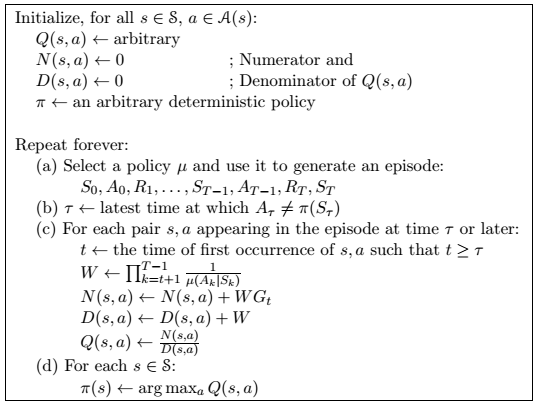
\includegraphics[scale=0.8]{offPolicyPseudo.png}
\caption{Off-Policy Monte Carlo Control Pseudo-code} \label{figure:offPolicy}
\end{figure}


\subsection{\textbf {Sarsa}}
Sarsa is an on-policy method based on model-free action policy estimation. It determines the optimal policy while controlling the MDP with respect to the algorithm which behaves according to the same policy that has been improved.

\subsection*{Sarsa On-Policy TD Control}
Sarsa is an on-policy method of TD learning, whose name is derived from the quintuple $Q(s_t, a_t, r_{t+1}, s_{t+1}, a_{t+1})$, where  $\mathbf{s_t, a_t}$ are the original state and action, $\mathbf{r_{t+1}}$ is the reward observed in the following state and $\mathbf{s_{t+1}, a_{t+1}}$ are the new state-action pair. It expresses the transition from one state-action pair to the next and its update rule is as follow:
\begin{align}
Q(s_t, a_t) \gets Q(s_t, a_t)+\alpha[r_{t+1}+\gamma Q(s_{t+1}, a_{t+1})-Q(s_t, a_t)]
\end{align}\\
The algorithm for Sarsa is presented in Figure 2.3 below:
\begin{figure}[H] \centering
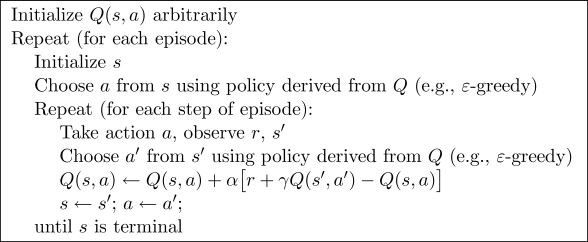
\includegraphics[scale=0.6]{sarsa_algorithm.png}
\caption{Sarsa Pseudo-code} \label{figure:Sarsa}
\end{figure}
As in all on-policy methods, we continually estimate $Q^\pi$ for the behavior policy $\pi$, and at the same time change $\pi$ toward greediness with respect to $Q^\pi$. The update is done after every transition from a nonterminal state $s$. If $s'$ is terminal, then $Q(s',a')$ will be defined as zero. \\
Regarding both Q-learning and Sarsa methods, the major difference between them is that the maximum reward for the next state is not necessarily used for updating the Q-values.

\subsection{\textbf {Q-learning}}
Q-learning is a model-free method which works by learning an action-value function that ultimately gives the expected utility of taking a given action in a given state and following the optimal policy thereafter.  The optimal policy can be constructed by selecting the action with the highest value in each state.
\subsection*{Q-learning Off-policy TD Control}
Q-learning is an off-policy TD control algorithm. It directly approximates the optimal policy $Q^*$ independent from the policy being followed. Its update rule is as follows:
\begin{align}
Q(s_t,a_t) \leftarrow Q(s_t,a_t)+\alpha[r_{t+1}+\gamma \max_a Q(s_{t+1},a)-Q(s_t,a_t)]
\end{align}
The influence of the policy is still in determining which state-action pairs are visited and updated. However, as long as all pairs continue to be updated, which is the minimal requirement to find optimal behavior in the general case, correct convergence shall be reached. Convergence to $Q^*$ with a probability of 1, requires stochastic approximation conditions on the sequence of step-size parameters, i.e. discounted $\epsilon$, $\alpha$. The algorithm is presented in Figure $\ref{figure:Q}$ below:
\begin{figure}[H] \centering
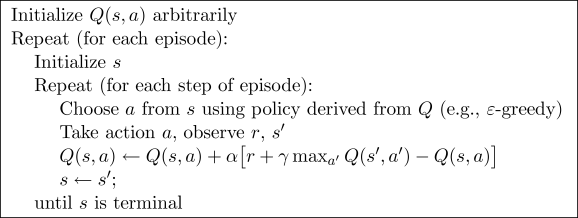
\includegraphics[scale=0.6]{pseudotmp9.png}
\caption{Q-learning: An off-policy TD control algorithm.} \label{figure:Q}
\end{figure}

\subsection{Reducing the state space}
\label{reduce}
Regard the current maximum statespace in the form of 
\begin{align}
statespace[predator(x_i,y_j), prey(x_k,y_l)]
\end{align}
This statespace has size $11^4$, spanning all possible positions of predator and prey in the $11 \times 11$ grid. Reducing the statespace would mean compressing this table without information loss. Notice the tables of policy and value iteration, table $\ref{pitS}$ and table $\ref{vitS}$, both displaying the values for all possible states by keeping the prey fixed at [5][5]. We can see the same value distribution; and a pattern where the values are proportional to the distance of the predator to the prey. When we look at table $\ref{rVIt}$, where the prey is at [3][2], we notice the exact same value distribution, only translated to the current position of the prey. 

\indent So a way of reducing the statespace would be by eliminating the representation of the prey within the statespace, by keeping it fixed; we marginalize the conditioning of the prey on the statevalue distribution. We can do this without information loss, by making use of a transform function which translates the actual positions of the prey and predator to an arbitrary one, where the position of the prey has been kept fixed; a statespace where only the position of the predator is variable. In our implementation we make use of one represented by table $\ref{vitS}$.

\indent The transform function hereby is a simple translation in the following form:
\begin{align}
\begin{split}
P'_{pred} &= \omega((P'_{prey}-P_{prey})+P_{pred}))
\qquad
\begin{cases}
P'_{pred} &= \text{Projected predator position} \\
P'_{prey} &= \text{Projected prey postion, [5][5] in our case} \\
P_{prey} &= \text{Actual prey position} \\
P_{pred} &= \text{Actual predator position}
\end{cases}
\end{split}
\end{align}
$\omega$ is the wrapper function implemented in our Position class, which takes into consideration that the grid is toroidal. 
Take table $\ref{rVIt}$ as an aid to illustrate this translation, where we pick position [1][5] as $P_{pred}$ having a certain value (6.440 for the actual state value would not yet be known in the reduced space scenario). [3][2], denotes $P_{prey}$. The value of the state[1][5][3][2] can be looked up by translating this to the calculated reduced space:
\begin{align}
\begin{split}
P'_{pred}
&=\omega((\begin{bmatrix} 
5 \\
5
\end{bmatrix} -
\begin{bmatrix}
3 \\
2
\end{bmatrix} )+
\begin{bmatrix}
1 \\
5
\end{bmatrix}
\end{split})
=
\begin{bmatrix}
3 \\
8
\end{bmatrix}
\end{align}
In the calculated reduced space this projected state[3][8][5][5], which has the same relative position of the predator to the prey as in the actual state, conforms with it's value 6.440, the same as we would in a maximum state space scenario. The reduced state space, effectively sized down to $11^2$, results in a lot less memory requirements as well as less computation, which leads us to a faster runtime as seen in table~\ref{runtime}. 

\begin{table}[H]
\caption{Runtime of normal and reduced statespace in seconds}
\centering
    \begin{tabular}{|l || l || l |}
    \hline
    Policy & Normal & Reduced \\ \hline
    Policy Evaluation & 13.04 & 0.35\\ \hline
    Policy Iteration & 28.27 & 0.28 \\ \hline
    Value Iteration & 4.13 & 0.27 \\
    \hline
    \end{tabular}
    \label{runtime}
\end{table}

\begin{table}[H]
\caption{Values from value iteration when the prey is at [3][2]}
\centering
\begin{tabular}{l|l*{9}{c}r}
  \hline
 & 0 & 1 & 2 & 3 & 4 & 5 & 6 & 7 & 8 & 9 & 10 \\ \hline 
0 & 6.440 & 7.148 & 7.936 & 8.780 & 7.936 & 7.148 & 6.440 & 5.802 & 5.237 & 5.237 & 5.802 \\
1 & 7.148 & 7.936 & 8.780 & 10.000 & 8.780 & 7.936 & 7.148 & 6.436 & 5.792 & 5.792 & 6.436 \\
2 & 7.839 & 8.780 & 10.000 & 0.000 & 10.000 & 8.780 & 7.839 & 6.997 & 6.251 & 6.251 & 6.997 \\
3 & 7.148 & 7.936 & 8.780 & 10.000 & 8.780 & 7.936 & 7.148 & 6.436 & 5.792 & 5.792 & 6.436 \\
4 & 6.440 & 7.148 & 7.936 & 8.780 & 7.936 & 7.148 & 6.440 & 5.802 & 5.237 & 5.237 & 5.802 \\
5 & 5.802 & 6.440 & 7.148 & 7.839 & 7.148 & 6.440 & 5.802 & 5.228 & 4.742 & 4.742 & 5.228 \\
6 & 5.228 & 5.802 & 6.436 & 6.997 & 6.436 & 5.802 & 5.228 & 4.712 & 4.291 & 4.291 & 4.712 \\
7 & 4.742 & 5.237 & 5.792 & 6.251 & 5.792 & 5.237 & 4.742 & 4.291 & 3.883 & 3.883 & 4.291 \\
8 & 4.742 & 5.237 & 5.792 & 6.251 & 5.792 & 5.237 & 4.742 & 4.291 & 3.883 & 3.883 & 4.291 \\
9 & 5.228 & 5.802 & 6.436 & 6.997 & 6.436 & 5.802 & 5.228 & 4.712 & 4.291 & 4.291 & 4.712 \\
10&5.802 & 6.440 & 7.148 & 7.839 & 7.148 & 6.440 & 5.802 & 5.228 & 4.742 & 4.742 & 5.228
\end{tabular}
\label{rVIt}
\end{table}
%\label{trans}

\section{Experiments and Results}
\label{results}

\subsection{Theoretical Differences}

\subsection{On-Policy Monte Carlo Control}

\subsection{Off-Policy Monte Carlo Control}
The purpose of this experiment was to implement Off-Policy Monte Carlo Control algorithm and to observe the results in terms of the target policy, maximum action value function, and also the number of step that the predator take to catch the prey. Different fix value of $\epsilon$ also been tested to show how this value, which represents the probability of exploring and exploiting, affect the learning processes of action value function. We also tried another approaches beside fix value to set the $\epsilon$ of the behavior policy in order to get a better results. We organize this subsection starting from presenting the results of using different fix values of $\epsilon$, then we will describe how different approach of setting $\epsilon$ value will affect the learning, and finally we will show the convergence of the target policy. 

\subsubsection*{Experiment with different values of $\epsilon$}
In this part we made some experiments by changing the fix value of $\epsilon$. Since the epsilon represents the chance of exploring and exploiting in learning, then we will make a conclusion related to that matter. 

The values that we tested was 0.5, 0.3, 0.1, and 0.001, and the result is shown by figure $\ref{figure:differentFixEpsilon}$ below. 
\begin{figure}[H] \centering
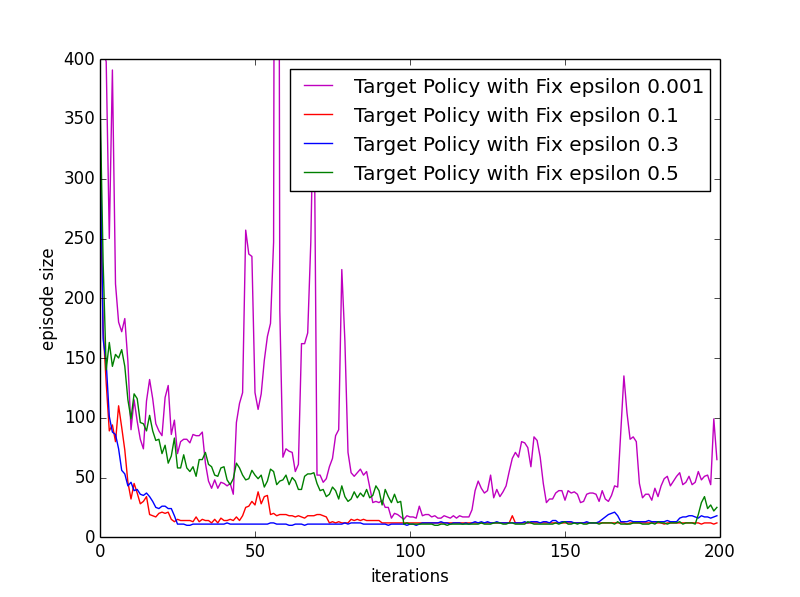
\includegraphics[scale=0.7]{target_fix_different_epsilon4.png}
\caption{Catching time with different fixed epsilon value} \label{figure:differentFixEpsilon}
\end{figure}

The figure above tells us that in our test case, $\epsilon$ value of 0.1 and 0.3 give the best performance, while 0.5 result shows a slower convergence than the previous values and 0.001 become the worst. This result con

\subsubsection*{Experiment with different approaches of setting $\epsilon$ value}
Firstly we set the $\epsilon$ value in $\epsilon$-greedy policy as a fix number, then we tried a different approach by making it dynamic by reducing the value after each fix number of iterations. The idea behind this approach was to put more chance in exploration at the beginning and slowly reduced the chance thus it started to exploit more time after time, but also maintained it to be stochastic in order to keep the learning process run.

Figure $\ref{figure:fixEpsilon}$ shows the number of steps the predator took to catch the prey in every iteration governed by the target policy. The $\epsilon$ value was set to be fix of 0.1. In order to get a consistent measurement, the episodes were generated from fix start points of the predator and the prey, which were (0,0) and (5,5) respectively. The time that the predator took to catch the prey can be used to measure the performance of Off-Policy Monte Carlo Learning after each iteration, because the target policy uses the $Q$ value immediately after each iteration. Since the target policy was greedy, then it always take best action based on the $Q$ value. The better the $Q$ value, the better target policy's performance should be.

\begin{figure}[H] \centering
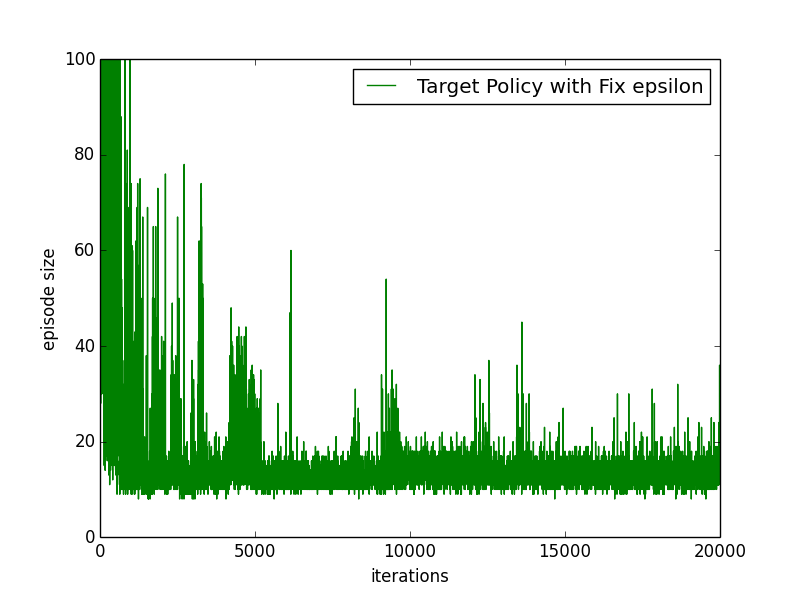
\includegraphics[scale=0.5]{target_fix_0_1.png}
\caption{Catch time with fix epsilon value} \label{figure:fixEpsilon}
\end{figure}

\begin{figure}[H] \centering
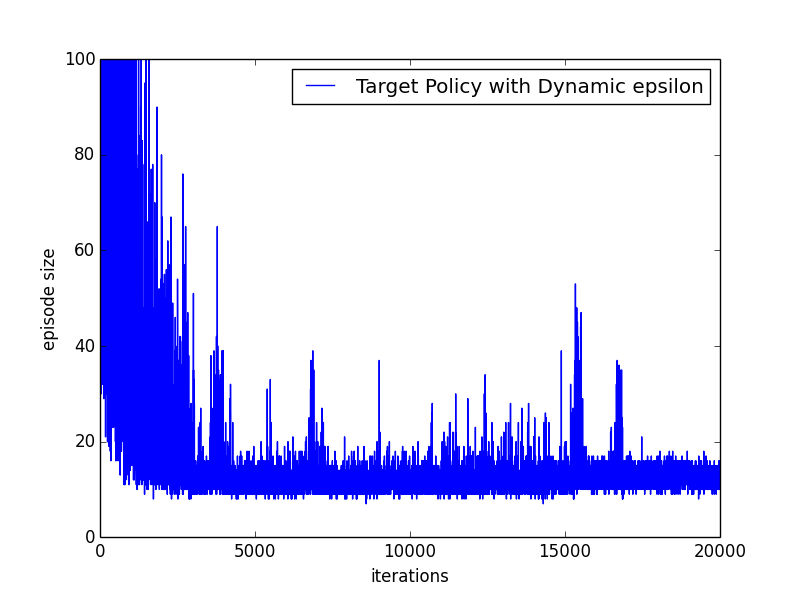
\includegraphics[scale=0.5]{target_dynamic_0_5_0_8_0_05.png}
\caption{Catching time with dynamic epsilon value}\label{figure:dynamicEpsilon} \label{figure:dynamicEpsilon}
\end{figure}

Figure $\ref{figure:dynamicEpsilon}$ was generated from the same setting as before except the value of $\epsilon$ was set to dynamically changed over iteration. First we set the value to 0.5 then after every 500 iterations it was reduced by multiplying with 0.8. In order to maintain the value not become too small, we set the minimum value to 0.1, because if $\epsilon$ is too small then it will become greedy and almost never explore anymore. As a consequence, learning processes will stop because both behavior and target policy always agree on actions taken in the generated episodes.

Even though the difference between the two figures above is not very significant, but we can still see the influence of setting the $\epsilon$ value to a fix and to a dynamic value. For fix value approach, the number of time drop quicker than the one from dynamic approach. This is because the fix value approach exploited more even from beginning due to the probability of exploiting much larger than exploring. On the other hand,the dynamic approach give the same probability between exploiting and exploring, so at the beginning it explored more than the fix value approach. Now let us see the last 3000 iterations from the two figures, it can be seen that dynamic value approach shows a slightly better performance, it fluctuates less than that in the other figure. Give more chance to explore at the beginning might help the learning process to find the optimal value slightly faster.

{\raggedleft{}Some text flushed right.}



\begin{figure}[H] \centering
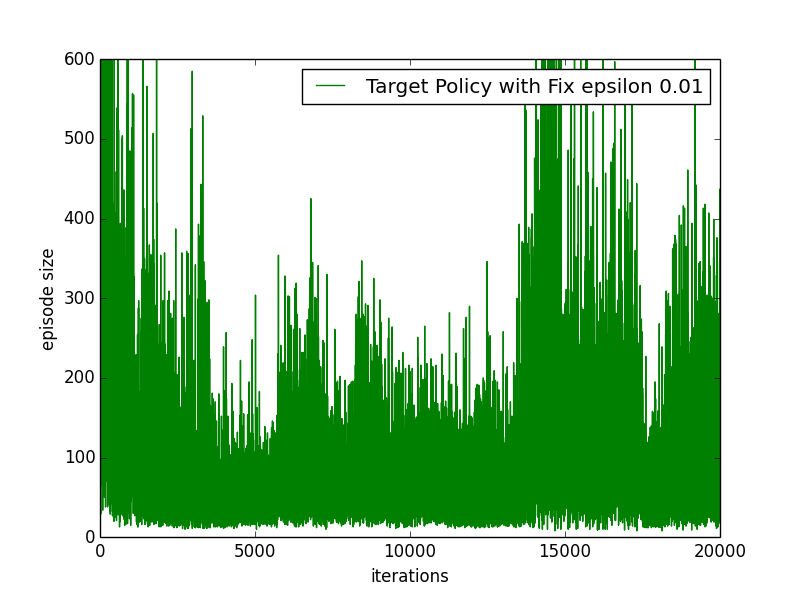
\includegraphics[scale=0.5]{target_fix_0_001.png}
\caption{Catch time with dynamic epsilon value} 
\end{figure}

\subsubsection*{Convergence}
In this section we will show that the Off-Policy Monte Carlo Control method can converge to the optimal policy
\begin{table}[H]
\caption{Target Policy Off-Policy Monte Carlo Control}
\centering
\begin{tabular}{l|l*{9}{c}r}
  \hline
 & 0 & 1 & 2 & 3 & 4 & 5 & 6 & 7 & 8 & 9 & 10 \\ \hline 
0 & $\rightarrow$&	$\downarrow$&	$\downarrow$&	$\rightarrow$&	$\downarrow$&	$\downarrow$&	$\leftarrow$&	$\leftarrow$&	$\leftarrow$&	$\leftarrow$&	$\leftarrow$\\	
1&$\rightarrow$&	$\rightarrow$&	$\rightarrow$&	$\rightarrow$&	$\downarrow$&	$\downarrow$&	$\leftarrow$&	$\downarrow$&	$\leftarrow$&	$\leftarrow$&	$\leftarrow$	\\
2&$\downarrow$&	$\rightarrow$&	$\downarrow$&	$\rightarrow$&	$\downarrow$&	$\downarrow$&	$\downarrow$&	$\downarrow$&	$\leftarrow$&	$\leftarrow$&	$\downarrow$\\	
3&$\downarrow$	&$\downarrow$&	$\rightarrow$&	$\rightarrow$&	$\downarrow$&	$\downarrow$&	$\leftarrow$&	$\leftarrow$&	$\leftarrow$&	$\downarrow$&	$\downarrow$\\	
4&$\rightarrow$&	$\rightarrow$&	$\rightarrow$&	$\rightarrow$  &	$\downarrow$&	$\downarrow$&	$\downarrow$&	$\downarrow$&	$\downarrow$&	$\leftarrow$&	$\leftarrow$\\	
5&$\rightarrow$  &	$\rightarrow$  &	$\rightarrow$  &	$\rightarrow$ &	$\rightarrow$ &	P&	$\leftarrow$&	$\leftarrow$&	$\leftarrow$&	$\leftarrow$&	$\leftarrow$\\	
6&$\rightarrow$ &	$\rightarrow$ &	$\uparrow$&	$\rightarrow$ &	$\rightarrow$ &	$\uparrow$&	$\leftarrow$&	$\leftarrow$&	$\leftarrow$&	$\uparrow$&	$\leftarrow$\\	
7&$\rightarrow$ &	$\rightarrow$ &	$\rightarrow$ &	$\uparrow$&	$\rightarrow$ &	$\uparrow$&	$\uparrow$&	$\leftarrow$&	$\leftarrow$&	$\leftarrow$&	$\leftarrow$\\	
8&$\uparrow$&	$\rightarrow$ &	$\uparrow$&	$\uparrow$&	$\uparrow$&	$\uparrow$&	$\uparrow$&	$\leftarrow$&	$\leftarrow$&	$\leftarrow$&	$\leftarrow$\\	
9&$\rightarrow$ &	$\uparrow$&	$\uparrow$&	$\rightarrow$ &	$\uparrow$&	$\uparrow$&	$\uparrow$&	$\leftarrow$&	$\leftarrow$&	$\uparrow$&	$\uparrow$\\	
10&$\uparrow$&	$\uparrow$&	$\rightarrow$ &	$\uparrow$&	$\uparrow$&	$\uparrow$&	$\uparrow$&	$\leftarrow$&	$\leftarrow$&	$\leftarrow$&	$\leftarrow$
\end{tabular}
\label{table:TargetPolicy}
\end{table}

The goal of the experiment in this algorithm was to evaluate the arbitrary policy, and to measure the number of iterations it took to converge. There were two parameters that should be defined, the discount factor $\mathbf{\gamma}$ and a threshold value for the stopping condition $\mathbf{\theta}$. The values of the parameters along with some results are shown in the following table.
\begin{table}[H]
\caption{Policy evaluation results}
\label{PE parameter}
\centering
    \begin{tabular}{| l || l |}
    \hline
      & Summary \\ \hline
    $\gamma$ & 0.8 \\ \hline
    $\theta$ & 1.0E-20 \\ \hline
    %runtime & 12248712457 ns \\ \hline
    Number of iterations & 106 \\
    \hline
    \end{tabular} 
\end{table}
%Runtime is time that the algorithm took to converge, and it was measured in nanosecond. While 
The number of iterations is the number of sweeps (sweep is a backup operation for all states) until it achieved convergence.
\begin{table}[H]
\caption{State values for the following states}
\label{PE states values}
\centering
\begin{tabular}{| l  |  l || c | r |}
  \hline
  Predator & Prey & $V(s)$ \\ \hline
  (0,0) & (5,5) & 0.005724141401102873 \\ \hline
  (2,3) & (5,4) & 0.18195076385152237 \\ \hline
  (2,10) & (10,10) & 0.18195076385152237 \\ \hline
  (10,10) & (0,0) & 1.1945854778368172 \\
  \hline  
\end{tabular}
\end{table}
In our test environment, the goal of the planning is to make the predator catch the prey as fast as possible. So state-value functions in this case represent how close the predator is from the prey in a given state. The closer the predator is from the prey, the higher the state-value function should be for that state. Table $\ref{PE states values}$ shows the state-value functions for four different states after performing iterative policy evaluation with parameters given in table $\ref{PE parameter}$.

The results make sense because the state value is proportional to the Manhattan distance between the predator and the prey. Intuitively the predator has a higher chance of catching the prey when it's closer.

%Based on the definition of the state-value function mentioned above, we will try to interpret the results and analyse whether they match the definition or not. We start with the first result where the predator's position is (0,0) and the prey's is (5,5). The shortest path of the predator in order to catch the prey is 10 steps. For now we can not say much about it's value except it is the smallest value among the others, but we will know it in a moment. Now we go to the second ones, where the predator is in cube (2,3) and the prey is in (5,4). The minimum steps from the predator's position to the prey's is 4 steps. It can be seen from the table that the $V(s)$ of the second result is higher than that in the first one, we consider these as a reasonable result respect to the number of minimum steps separated the predator from the prey. From the third result, we got the same $V(s)$ from the previous one, but at the first glance it seems that the distance from the predator to the prey are longer than that in the previous one. One thing to remember is that the grid of the environment is toroidal, so the minimum steps from (2,10) to (10,10) is actually 4 steps, so it is again make sense to have the same value of $V(s)$ with the previous one. The last result has the biggest $V(s)$ value, since it is the closest position of the predator from the prey. The number of minimum steps is only 2 due to toroidal grid. So, with all of these reasonable result, we can say that the algorithm performed correctly as intended.


\subsection{Policy Iteration}
For all the experiments with policy iteration theta was defined as $\theta = 1.0E^{-20}$, in order to perform a thorough sanity check, as it was suggested. As far as convergence is concerned it is presented in table~\ref{convPIter}, and as we can see for larger values of $\gamma$ convergence is slower since more iterations are needed because $\Delta$ is smaller and it takes longer to reach $\theta$.

\begin{table}[H]
\caption{Convergence in iterations for different $\gamma$}
\centering
\begin{tabular}{|l||c|c|}
\hline
$\gamma$&Evaluation runs&Improvement runs\\
\hline
0.1&100&8\\
\hline
0.5&227&7\\
\hline
0.7&323&8\\
\hline
0.9&763&10\\
\hline
\end{tabular}
\label{convPIter}
\end{table}


Following a similar notion as in policy evaluation we present the state-value table in ~\ref{pitS} for the states that are composed from the prey being at position prey(5,5). As in the case of policy evaluation the state values are proportional to the distance between the predator and the prey. The closer to the prey the higher the value. As we can also see the position of the prey is defined as the goal to be reached, hence the value will be 0 since there aren't any successor states and the episode ends.

\begin{table}[H]
\caption{Values from policy iteration when the prey is at [5][5]}
\centering
\begin{tabular}{l|l*{9}{c}r}
  \hline
   & 0 & 1 & 2 & 3 & 4 & 5 & 6 & 7 & 8 & 9 & 10 \\ \hline 
0 & 3.883 & 4.291 & 4.742 & 5.237 & 5.792 & 6.251 & 5.792 & 5.237 & 4.742 & 4.291 & 3.883  \\
1 & 4.291 & 4.712 & 5.228 & 5.802 & 6.436 & 6.997 & 6.436 & 5.802 & 5.228 & 4.712 & 4.291  \\
2 & 4.742 & 5.228 & 5.802 & 6.440 & 7.148 & 7.839 & 7.148 & 6.440 & 5.802 & 5.228 & 4.742  \\
3 & 5.237 & 5.802 & 6.440 & 7.148 & 7.936 & 8.780 & 7.936 & 7.148 & 6.440 & 5.802 & 5.237  \\
4 & 5.792 & 6.436 & 7.148 & 7.936 & 8.780 & 10.000 & 8.780 & 7.936 & 7.148 & 6.436 & 5.792  \\
5 & 6.251 & 6.997 & 7.839 & 8.780 & 10.000 & 0.000 & 10.000 & 8.780 & 7.839 & 6.997 & 6.251  \\
6 & 5.792 & 6.436 & 7.148 & 7.936 & 8.780 & 10.000 & 8.780 & 7.936 & 7.148 & 6.436 & 5.792  \\
7 & 5.237 & 5.802 & 6.440 & 7.148 & 7.936 & 8.780 & 7.936 & 7.148 & 6.440 & 5.802 & 5.237  \\
8 & 4.742 & 5.228 & 5.802 & 6.440 & 7.148 & 7.839 & 7.148 & 6.440 & 5.802 & 5.228 & 4.742  \\
9 & 4.291 & 4.712 & 5.228 & 5.802 & 6.436 & 6.997 & 6.436 & 5.802 & 5.228 & 4.712 & 4.291  \\
10&3.883 & 4.291 & 4.742 & 5.237 & 5.792 & 6.251 & 5.792 & 5.237 & 4.742 & 4.291 & 3.883
\end{tabular}
\label{pitS}
\end{table}

\subsection{Value Iteration}
As in policy iteration, similar tables, namely ~\ref{convVIter}, ~\ref{vitS}, for value iteration are presented, with $theta = 1.0E^{-20}$. 
\begin{table}[H]
\caption{Convergence in iterations for different $\gamma$}
\centering
\begin{tabular}{|l||r|}
\hline
$\gamma$ & Nr. of iterations\\
\hline
0.1& 18\\
\hline
0.5& 25\\
\hline
0.7& 27\\
\hline
0.9& 29\\
\hline
\end{tabular}
\label{convVIter}
\end{table}

\begin{table}[H]
\caption{Values from value iteration when the prey is at [5][5]}
\centering
\begin{tabular}{l|l*{9}{c}r}
  \hline
 & 0 & 1 & 2 & 3 & 4 & 5 & 6 & 7 & 8 & 9 & 10 \\ \hline 
0 & 3.883 & 4.291 & 4.742 & 5.237 & 5.792 & 6.251 & 5.792 & 5.237 & 4.742 & 4.291 & 3.883 \\
1 & 4.291 & 4.712 & 5.228 & 5.802 & 6.436 & 6.997 & 6.436 & 5.802 & 5.228 & 4.712 & 4.291 \\
2 & 4.742 & 5.228 & 5.802 & 6.440 & 7.148 & 7.839 & 7.148 & 6.440 & 5.802 & 5.228 & 4.742 \\
3 & 5.237 & 5.802 & 6.440 & 7.148 & 7.936 & 8.780 & 7.936 & 7.148 & 6.440 & 5.802 & 5.237 \\
4 & 5.792 & 6.436 & 7.148 & 7.936 & 8.780 & 10.000 & 8.780 & 7.936 & 7.148 & 6.436 & 5.792 \\
5 & 6.251 & 6.997 & 7.839 & 8.780 & 10.000 & 0.000 & 10.000 & 8.780 & 7.839 & 6.997 & 6.251 \\
6 & 5.792 & 6.436 & 7.148 & 7.936 & 8.780 & 10.000 & 8.780 & 7.936 & 7.148 & 6.436 & 5.792 \\
7 & 5.237 & 5.802 & 6.440 & 7.148 & 7.936 & 8.780 & 7.936 & 7.148 & 6.440 & 5.802 & 5.237 \\
8 & 4.742 & 5.228 & 5.802 & 6.440 & 7.148 & 7.839 & 7.148 & 6.440 & 5.802 & 5.228 & 4.742 \\
9& 4.291 & 4.712 & 5.228 & 5.802 & 6.436 & 6.997 & 6.436 & 5.802 & 5.228 & 4.712 & 4.291 \\
10& 3.883 & 4.291 & 4.742 & 5.237 & 5.792 & 6.251 & 5.792 & 5.237 & 4.742 & 4.291 & 3.883
\end{tabular}
\label{vitS}
\end{table}

\subsection{Comparison of Policy and Value iteration}
We can see that tables ~\ref{pitS}  and ~\ref{vitS} have the same values, and that can be explained because both methods converge to the optimal policy. The only difference can be the number of iterations it takes to converge to that optimal policy. Value iteration has only one backup operation for each state and reduces the policy evaluation to one step, whereas policy iteration performs multiple evaluations until it reaches the improvement part. That's why it will converge much faster than policy iteration which can be shown in graph~\ref{converge}. 

\begin{figure}[H] \centering
%\fbox{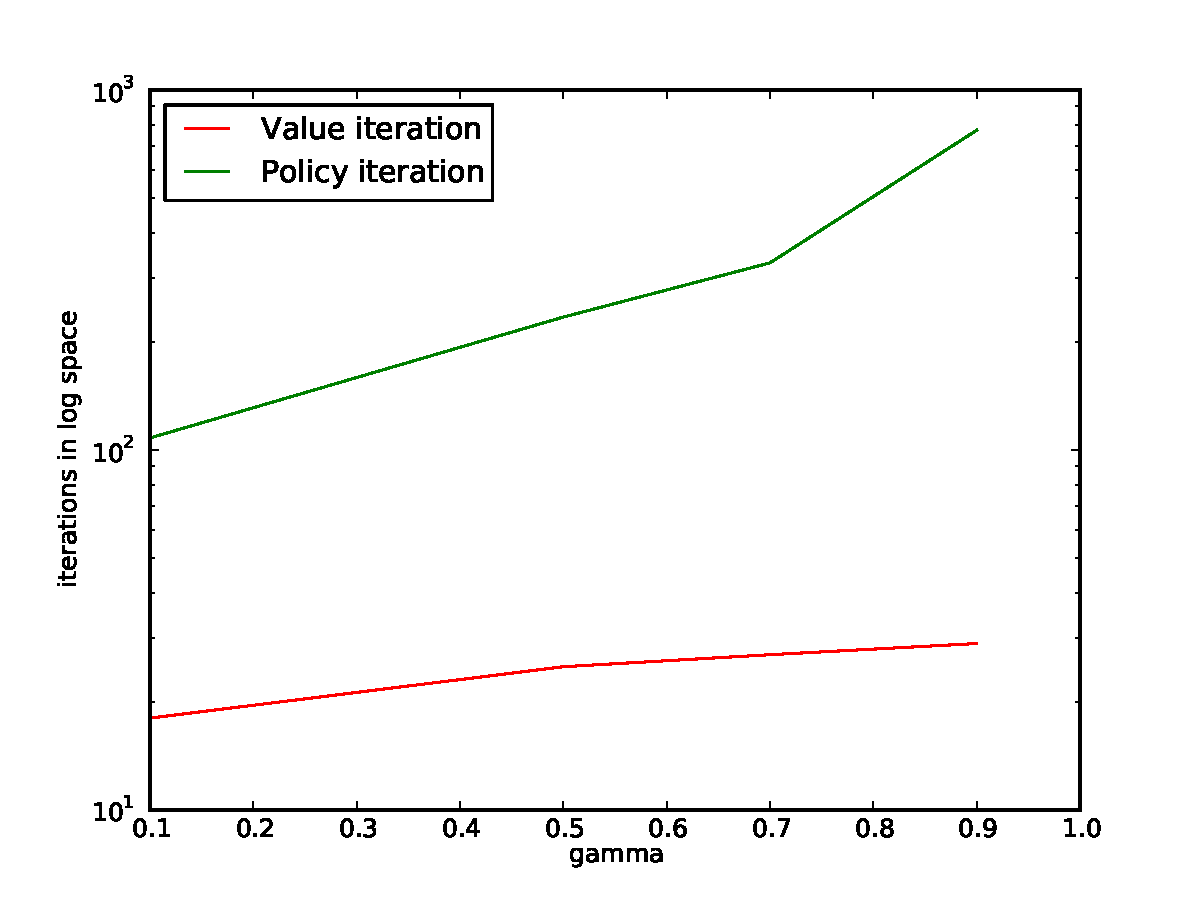
\includegraphics[scale=0.5]{convergence.pdf}}
\caption{Comparative graph of convergence for policy and value iteration} \label{converge}
\end{figure}

\section{conclusion}
\label{discussion}
To conclude we presented the algorithms of policy evaluation, policy iteration, value iteration as well as their results on a predator-prey environment which consists of a toroidal grid. Through the presentation of those results we gained better insights on the advantages and disadvantages of using a specific algorithm. In our assignment value iteration converges faster to the optimal policy than policy iteration, and seems to be better in that regard. However maybe in some specific problems we need a decoupling of policy evaluation from improvement, because further evaluation is not needed. This can only be done with policy iteration.

Additionally, we reduced the statespace from $11^4$ states to $11^2$ states and we can actually reduce it even more, and we plan to try it for assignment 2, ie a quarter of that same statespace by employing mirroring. The idea came from the visualization of the distribution of values of the states around the projected prey. It is not as straightforward as the transformation used in the initial reduction because state actions need to be mirrored as well.

%we are relied to a complete and finite MDP
%see the big picture of GPI loop 



\begin{thebibliography}{9}

\bibitem{suttonBarto}
  Richard S. Sutton, Andrew G. Barto,
  \emph{Reinforcement Learning: An Introduction}.
  MIT Press, Cambridge, MA, 
  A Bradford Book,
  1998.

\end{thebibliography}

%%% End document
\end{document}

